\documentclass[tikz,border=12pt]{standalone}
\usepackage[T1]{fontenc}
\usepackage{mathpazo}
\usepackage{amsmath,amssymb}
\usetikzlibrary{arrows.meta, positioning, calc, decorations.pathreplacing}

\definecolor{stblue}{HTML}{7B97AD}
\definecolor{rwgold}{HTML}{B8995E}
\definecolor{sage}{HTML}{7A9A7E}
\definecolor{dkbrown}{HTML}{3D3530}
\definecolor{wmgray}{HTML}{7B7067}
\definecolor{cream}{HTML}{F9F6F0}
\definecolor{border}{HTML}{D4C9B8}
\definecolor{terracotta}{HTML}{C47A6A}
\definecolor{lavender}{HTML}{907EA0}

\begin{document}
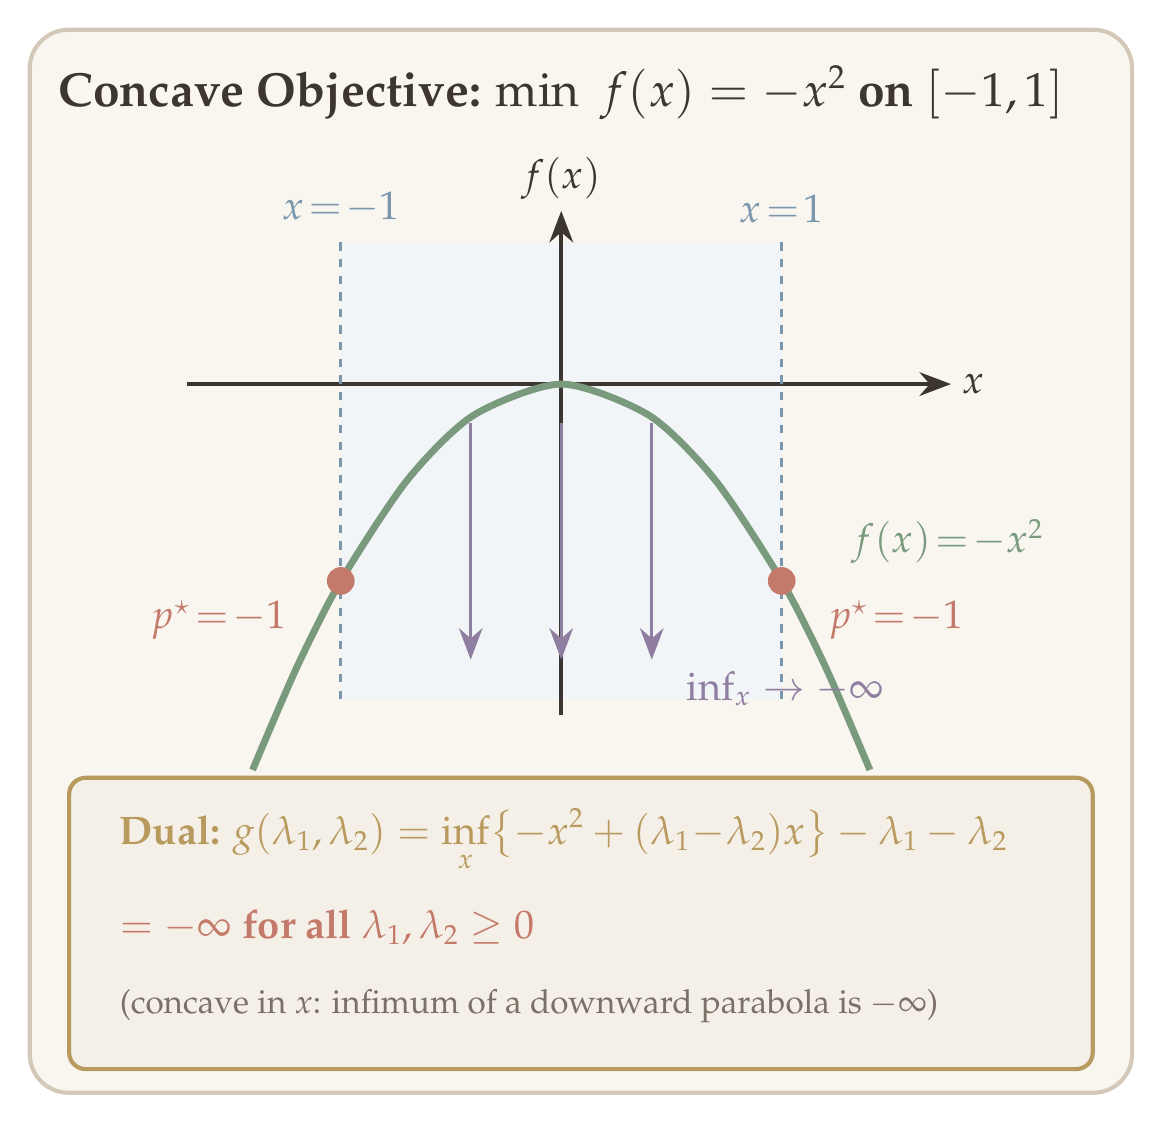
\begin{tikzpicture}[>={Stealth[length=4mm, width=3mm]}, line width=1.5pt]

% Background
\fill[cream, rounded corners=14pt] (-2.5,-5.0) rectangle (11.5,8.5);
\draw[border, line width=1.5pt, rounded corners=14pt] (-2.5,-5.0) rectangle (11.5,8.5);

% Title
\node[font=\LARGE\bfseries, text=dkbrown, align=center] at (4.25,7.7)
  {Concave Objective: $\min\; f(x)=-x^2$ on $[-1,1]$};

% Coordinate mapping:
%   real x in [-1.6, 1.6] -> tikz X:  center at 4.25, scale 2.8 per unit
%     tikz X = 4.25 + 2.8*x
%     x=-1.6 -> -0.23,  x=-1 -> 1.45,  x=0 -> 4.25,  x=1 -> 7.05,  x=1.6 -> 8.73
%   real f in [-1.5, 0.3] -> tikz Y:  f=0 at tikzY=4.0, scale 2.5 per unit
%     tikz Y = 4.0 + 2.5*f
%     f=0 -> 4.0,  f=-1 -> 1.5,  f=-1.5 -> 0.25

% Feasible region [-1, 1] shading (drawn before axes so it doesn't eclipse them)
\fill[stblue!10] (1.45,0.0) rectangle (7.05,5.8);

% Axes
\draw[->, dkbrown, line width=1.5pt] (-0.5,4.0) -- (9.2,4.0)
  node[right, font=\Large, text=dkbrown] {$x$};
\draw[->, dkbrown, line width=1.5pt] (4.25,-0.2) -- (4.25,6.2)
  node[above, font=\Large, text=dkbrown] {$f(x)$};

% Dashed vertical lines at x = -1 and x = 1
\draw[stblue, dashed, line width=1.2pt] (1.45,0.0) -- (1.45,5.8);
\draw[stblue, dashed, line width=1.2pt] (7.05,0.0) -- (7.05,5.8);
\node[font=\Large, text=stblue, anchor=south] at (1.45,5.9) {$x\!=\!-1$};
\node[font=\Large, text=stblue, anchor=south] at (7.05,5.9) {$x\!=\!1$};

% Plot f(x) = -x^2
% x=-1.4: f=-1.96  tikzX=0.33, tikzY=-0.9
% x=-1.2: f=-1.44  tikzX=0.89, tikzY=0.4
% x=-1.0: f=-1     tikzX=1.45, tikzY=1.5
% x=-0.7: f=-0.49  tikzX=2.29, tikzY=2.775
% x=-0.4: f=-0.16  tikzX=3.13, tikzY=3.6
% x=0:    f=0      tikzX=4.25, tikzY=4.0
% x=0.4:  f=-0.16  tikzX=5.37, tikzY=3.6
% x=0.7:  f=-0.49  tikzX=6.21, tikzY=2.775
% x=1.0:  f=-1     tikzX=7.05, tikzY=1.5
% x=1.2:  f=-1.44  tikzX=7.61, tikzY=0.4
% x=1.4:  f=-1.96  tikzX=8.17, tikzY=-0.9

\draw[sage, line width=2.5pt] plot[smooth, tension=0.45] coordinates {
  (0.33,-0.9) (0.89,0.4) (1.45,1.5) (2.29,2.775) (3.13,3.6) (4.25,4.0)
  (5.37,3.6) (6.21,2.775) (7.05,1.5) (7.61,0.4) (8.17,-0.9)
};

\node[font=\Large\bfseries, text=sage, anchor=west] at (7.8,2.0) {$f(x)\!=\!-x^2$};

% Mark p* = -1 at x = +-1 (endpoints)
\fill[terracotta] (1.45,1.5) circle (5pt);
\fill[terracotta] (7.05,1.5) circle (5pt);

% p* labels — offset to avoid overlapping the dashed lines and each other
\node[font=\Large\bfseries, text=terracotta, anchor=east] at (0.9,1.0)
  {$p^\star\!=\!-1$};
\node[font=\Large\bfseries, text=terracotta, anchor=west] at (7.5,1.0)
  {$p^\star\!=\!-1$};

% Illustration: downward arrows showing inf = -infty over unrestricted x
\foreach \xpos in {3.1, 4.25, 5.4} {
  \draw[lavender, line width=1.2pt, ->] (\xpos, 3.5) -- (\xpos, 0.5);
}
\node[font=\Large\itshape, text=lavender, anchor=north west] at (5.7,0.5) {$\inf_x \to -\infty$};

% Dual annotation box — below the plot, with breathing room
\draw[rwgold, line width=1.5pt, rounded corners=6pt] (-2.0,-4.7) rectangle (11.0,-1.0);
\fill[rwgold, opacity=0.06, rounded corners=6pt] (-2.0,-4.7) rectangle (11.0,-1.0);
\node[font=\Large\bfseries, text=rwgold, anchor=west] at (-1.5,-1.8)
  {Dual: $g(\lambda_1,\lambda_2) = \displaystyle\inf_{x}\bigl\{-x^2 + (\lambda_1\!-\!\lambda_2)x\bigr\} - \lambda_1 - \lambda_2$};
\node[font=\Large\bfseries, text=terracotta, anchor=west] at (-1.5,-2.9)
  {$= -\infty$ for all $\lambda_1,\lambda_2 \ge 0$};
\node[font=\large, text=wmgray, anchor=west] at (-1.5,-3.9)
  {(concave in $x$: infimum of a downward parabola is $-\infty$)};

\end{tikzpicture}
\end{document}
